\documentclass{beamer}
\usepackage[brazil]{babel}
\usepackage[utf8]{inputenc}
\usepackage{amsfonts}
\usepackage{amsmath}
\usepackage{float}
\usepackage{subfig}

\mode<presentation>
{
    \usetheme{PaloAlto}
    
    \setbeamercovered{transparent}
}

\title{Aplicação ARHydra}

%\subtitle{}

% - Use the \inst{?} command only if the authors have different
%   affiliation.
%\author{F.~Author\inst{1} \and S.~Another\inst{2}}
\author{Ricardo Felipe Lacerda de Andrade}
% - Use the \inst command only if there are several affiliations.
% - Keep it simple, no one is interested in your street address.

\institute[UnB]
{
    %\inst{1}
    Departamento de Ciência da Computação\\
    Instituto de Ciências Exatas\\
    Universidade de Brasília
}

\date{08 de outubro de 2012}

%
%\mode<beamer>{
%  \usetheme{JuanLesPins}
%}


\begin{document}

% ------------- TITLE PAGE -------------
\begin{frame}
\titlepage
\end{frame}
% ------------- TITLE PAGE -------------


% ------------- SUMARIO -------------
\begin{frame}
	\frametitle{Sumário}
	\tableofcontents
\end{frame}


% ------------- Introdução -------------

\section{Introdução}

	% ------------- Computação Ubíqua -------------

	\subsection{Computação Ubíqua}
		\begin{frame}
	    	\frametitle{Computação Ubíqua}
	    		\begin{itemize}
	    		  \item Integração dos computadores ao cotidiano dos seres humanos;
	    		  \item Utilização de ambientes inteligentes para integrar os dispostivos; 
	    		  \item Auxílio ao usuário em suas tarefas.  
	    		  %\item Permitir com que a interação entre o usuário e as tarefas a serem 
		      	  %		desempenhas ocorram de forma transparente.
	    		\end{itemize}
		\end{frame}
		
		\begin{frame}  
			\frametitle{Computação Ubíqua} 
		    	Possui as seguintes características:
		    	\begin{itemize}
		    	  \item Invisibilidade;
		    	  \item Sensibilidade ao contexto;
		    	  \item Pró-atividade.
		    	\end{itemize}
		\end{frame}
		
		\begin{frame}
			\frametitle{Níveis de interação}
			
			Há três níveis de interação:
			
			\begin{itemize}
			  \item Interação direta 
			  \item Interação sugerida 
			  \item Interação automática
			\end{itemize}
			
		\end{frame}
		
		\begin{frame}
			\frametitle{\emph{Middleware}}
			
			\begin{itemize}
				\item	Camadas de \emph{softwares} responsáveis por orquestrar a troca 
						de informações a respeito dos usuários e serviços inseridos no ambiente;
			
				\item 	Abstração detalhes de serviços de segurança, comunicação, identificação 
						de serviços, dentre outros.
			\end{itemize}
		\end{frame}
		
		%\begin{frame}
		%	\frametitle{\emph{Smart Space}}
		%    	É um ambiente onde a tecnologia ubíqua é utilizada para interagir de forma inteligente com o
		%    	usuário e prover facilidades em tarefas do dia a dia, provida pela integração de vários 
		%    	dispositivos e recursos.
		%\end{frame}
		
		%\begin{frame}
		%	\frametitle{\emph{Smart Space}}
		%		\begin{figure}[h]
		%		\centering 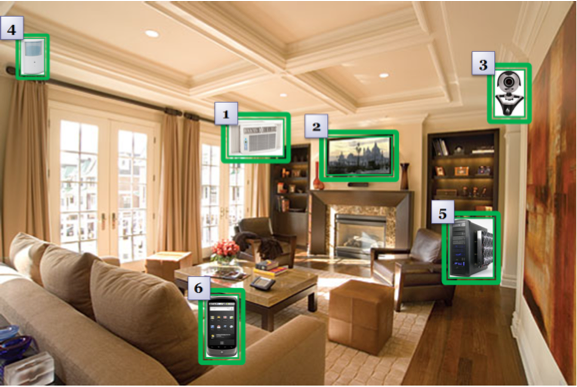
\includegraphics[scale=.45]{figuras/smartspace.png}
		%	\end{figure}
		%\end{frame}
		
	
		
		\subsection{uOS}
		\begin{frame}
			\frametitle{\emph{uOS}}
		%	\begin{block}{Definição} 
				\begin{itemize}
				  \item Adaptabilidade de serviços;
				  \item Utiliza protocolos ~\emph{uP};
				  \item Comunicação por drivers.
				\end{itemize}
		 %   \end{block}
		\end{frame}
		
		\subsection{Hydra}
		\begin{frame}
			\frametitle{Redirecionamento de recursos}
			
			\begin{figure}[h]
				\centering 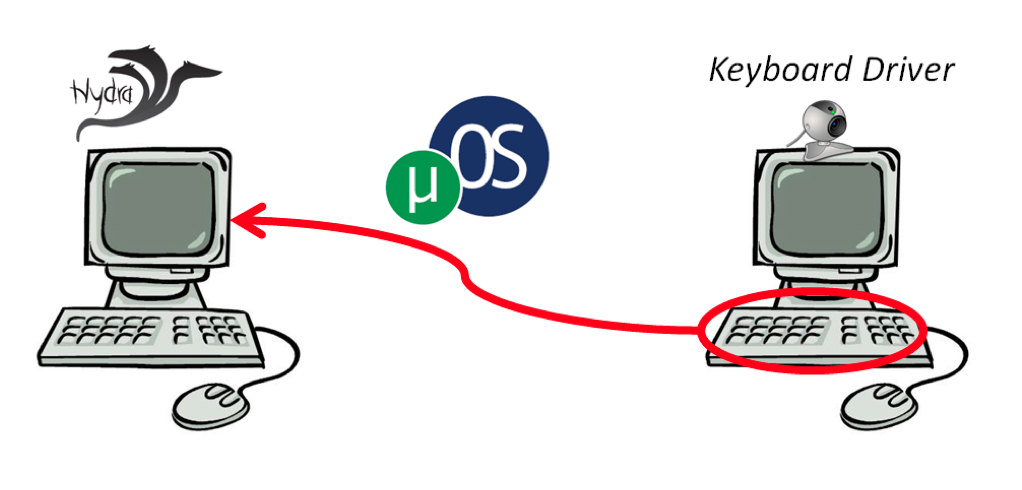
\includegraphics[scale=.25]{figuras/hydra_redirecionamento.png}
			\end{figure}
			%\begin{itemize}
			%  \item Tem por objetivo prover o redirecionamento de recursos;
			%  \item Suporte aos recursos de câmera, \emph{mouse}, teclado e tela.
			%  \item Nível sugerido de interação;
			%\end{itemize}
		\end{frame}
		
		\begin{frame}
			\frametitle{Hydra}
			
			\begin{itemize}
				\item É uma aplicação que possibilita o redirecionamento dos recursos, 
						utilizando o uOS para comunicar-se aos dispositivos; 
				\item Nível sugerido de interação;  
				\item Suporte aos recursos de câmera, \emph{mouse}, teclado e tela.
			\end{itemize}
		\end{frame}
		
		\begin{frame}
			\frametitle{Hydra}
			
			\begin{figure}[h]
				\centering 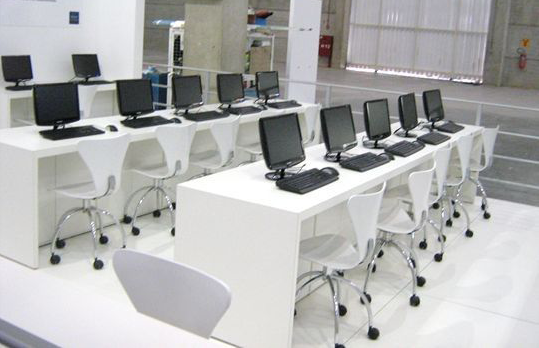
\includegraphics[scale=.5]{figuras/sala_computadores.png}
			\end{figure}
		\end{frame}


		
		\begin{frame}
			\frametitle{Hydra}
			
			\begin{figure}[h]
				\centering 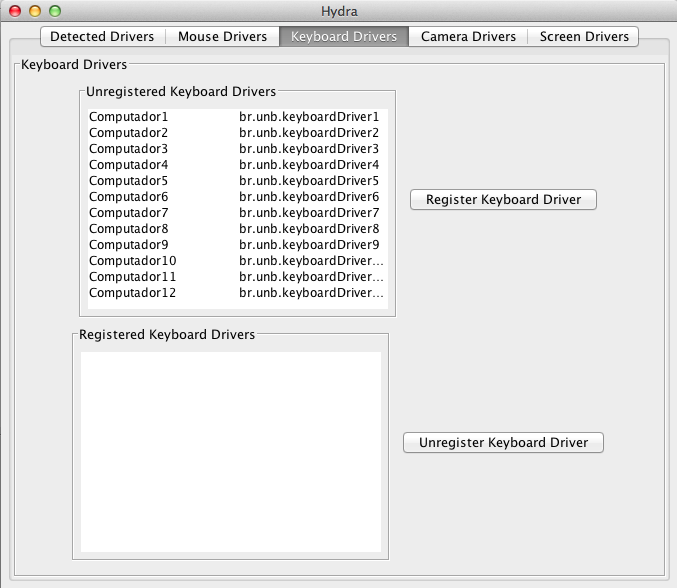
\includegraphics[scale=.35]{figuras/hydra_apresentacao.png}
			\end{figure}
		\end{frame}

% ------------- Problema -------------
\section{Problema}

	\begin{frame}
	    \frametitle{Problema}
	    Como identificar os recursos disponibilizados pelos dispositivos inseridos no \emph{smart space} 
	    de forma visual?
	\end{frame}		
    	
    	%O middleware fornece para as aplicações um código identificador de cada recurso 
    	%disponível no ambiente inteligente. No entanto, esse código 
    	
    	%O nível sugerido de interação pode ser melhorado devido ao fato do 
    	%middleware externalizar o nome dos recursos 
    	
	
% ------------- Hipotese -------------
\section{Hipótese}
	\begin{frame}
		\frametitle{Hipóteses e objetivos}
		
		O nível sugerido de interação, implementado na Hydra, pode ser melhorado 
		adicionando uma nova forma de identificação dos recursos disponíveis de um
		dispositivo, através do uso de técnicas de Realidade Aumentada. 
		
	\end{frame}		

% ------------- Realidade Aumentada -------------

\section{Realidade Aumentada}
	
	%\subsection{Realidade Aumentada}
	
		\begin{frame}
			\frametitle{Realidade Aumentada}
			Tem o objetivo de inserir novas informações utilizando objetos virtuais 
			que dizem respeito a objetos físicos visualizados pelo usuário.
		\end{frame}		

		\begin{frame}
				\frametitle{Realidade Aumentada}
				Possui as seguintes características:
				
				\begin{itemize}
				  \item Combinação entre o real e virtual;
				  \item Interatividade em tempo real;
				  \item Visualização dos objetos virtuais em 3D.
				\end{itemize}
		\end{frame}
		
		
		%\begin{frame}
		%	\frametitle{Marcadores na Realidade Aumentada}
		%	
		%	\begin{itemize}
		%	  \item São exemplos de aplicações voltadas para a Realidade Aumentada: 
		%	  		ARToolkit, ARTag e ARToolkitPlus;
		%	  \item Cada aplicação pode implementar seus próprios marcadores;
		%	  \item Os objetos virtuais são sobrepostos a esses marcadores,
		%	  		apresentando as informações correspondestes ao marcador para
		%	  		o usuário;
		%	  \item Também é possível apresentar os objetos virtuais utilizando 
		%	  		posições de altitude, latitude e longitude, denominado de 
		%	  		\emph{Point's Of Interest}. 
		%	\end{itemize}			
			
			
			%\begin{itemize}
			%  \item 
			%  \item Uma forma de mapear locais é feita através de POI's 
			%  		(\emph{Point's of Interest}).
			%\end{itemize}
			
		%\end{frame}
		
% ------------- ARHydra -------------

\section{ARHydra}

	\subsection{Conceitos}
	
	\begin{frame}
		\frametitle{ARHydra}
		
		
		\begin{itemize}
		  \item \emph{\textbf{A}ugmented \textbf{R}eality \textbf{Hydra}};
		  \item Objetivo de permitir ao usuário visualizar os recursos que
		  		estão sendo disponibilizados pelos dispositivos inseridos no
		  		ambiente inteligente e prover uma interface mais intuitiva para
		  		o redirecionamento dos recursos.
		\end{itemize}
	\end{frame}
	
	\begin{frame}
		\frametitle{Marcadores na Realidade Aumentada}
			
		\begin{figure}[h]
			\centering 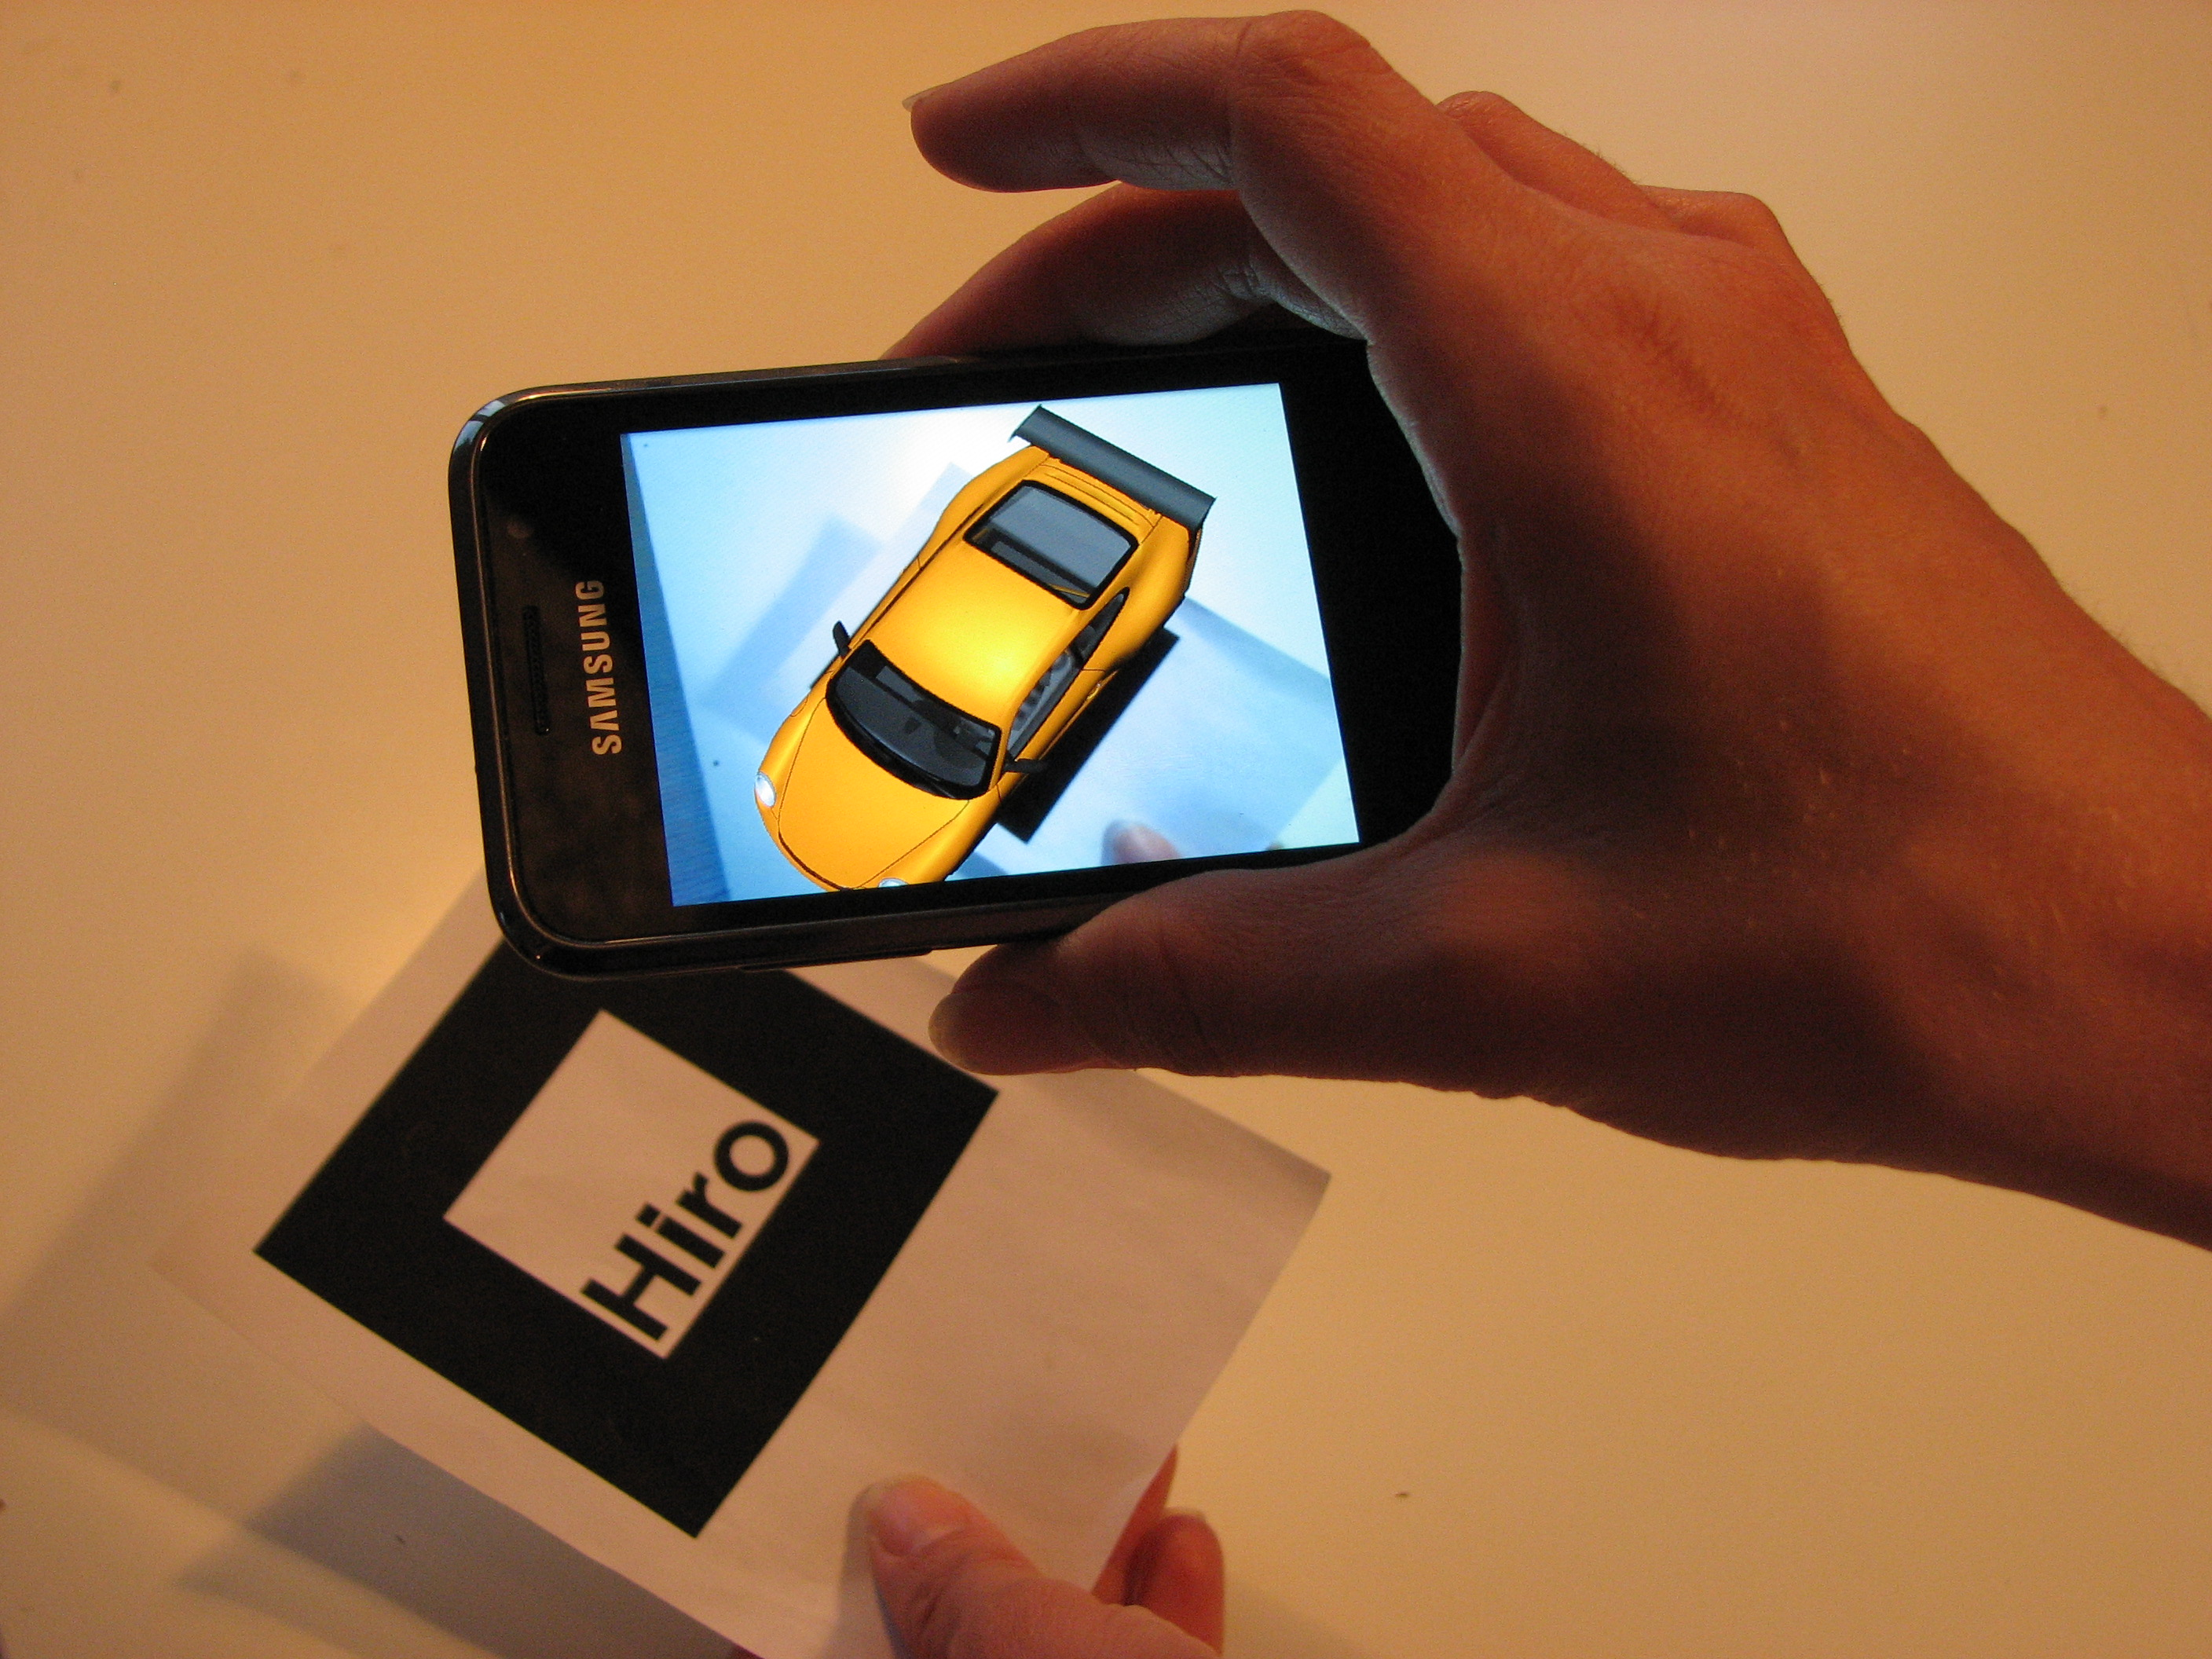
\includegraphics[scale=.07]{figuras/carro.jpg}
		\end{figure}
	\end{frame}
	
	\begin{frame}
		\frametitle{Marcador utilizado na ARHydra}
		\begin{figure}[htb]
			\begin{center}
					
\includegraphics[width=0.9\textwidth]{figuras/marcador_arhydra.png}
			\end{center}
		\end{figure}
	\end{frame}
	
	\begin{frame}
		\frametitle{Por que utilizar o QRCode?}
		\begin{itemize}
		  \item Possiblidade de inserção de informação através de texto;
		  \item Rápida leitura;
		  \item Implementa quatro níveis que possibilitam a recuperação a falhas.
		\end{itemize}
	\end{frame}
	
	
	%\subsection{Interação com o ambiente}
	%\begin{frame}
	%	\frametitle{Interação com o ambiente}
	%	\begin{figure}[htb]
	%		\begin{center}
	%				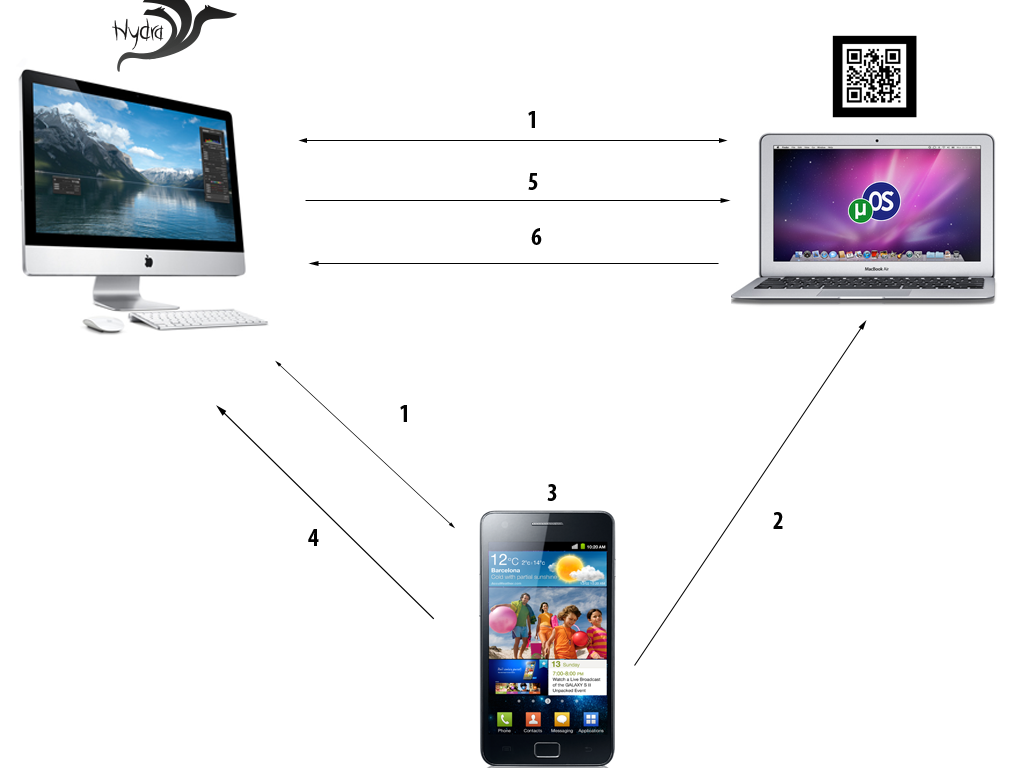
\includegraphics[width=0.8\textwidth]{figuras/integracao_arhydra.png}
	%		\end{center}
	%		\caption{Integração da ARHydra com o ambiente.}
	%		\label{fig:arhydra_integracao}
	%	\end{figure}
	%\end{frame}
	
	\subsection{Arquitetura}	
	\begin{frame}
		\frametitle{Arquitetura da ARHydra}
		
		A aplicação ARHydra se divide em quatro módulos:
		
		\begin{itemize}
		  \item \textbf{Reconhecimento}
		  \item \textbf{Decodificação}
		  \item \textbf{Integração}
		  \item \textbf{Apresentação}
		\end{itemize}
		
	\end{frame}
	
	
	\begin{frame}
		\frametitle{Interação entre os módulos}
		
		\begin{figure}[htb]
			\begin{center}
					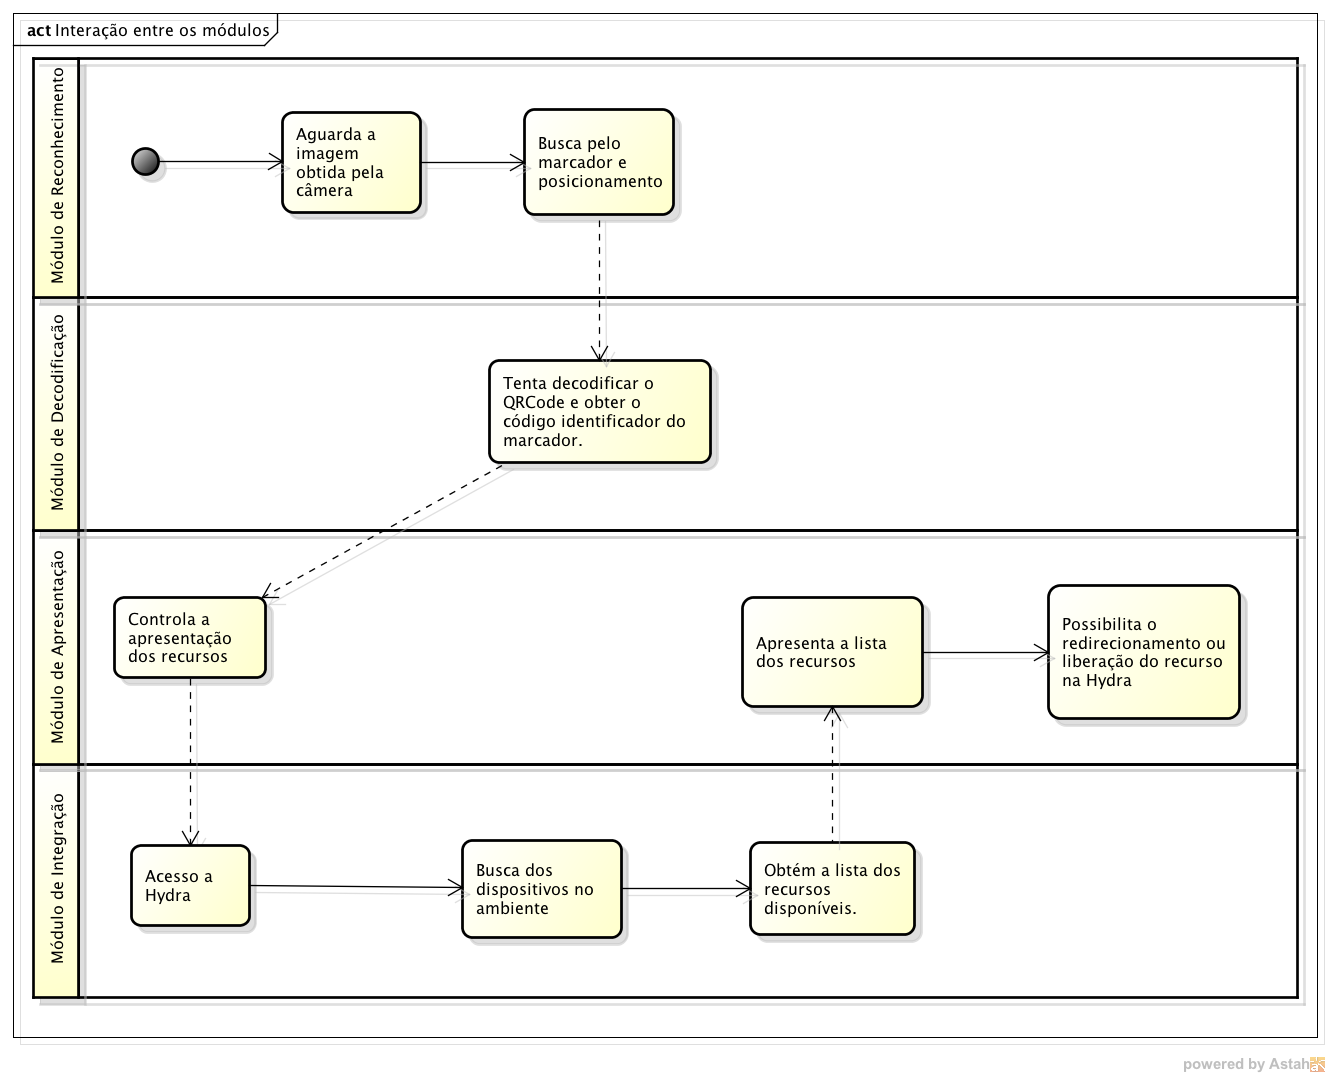
\includegraphics[width=0.9\textwidth]{figuras/interacao_modulos.png}
			\end{center}
		\end{figure}
	
	\end{frame}
		
	
	%\begin{frame}
	%	\frametitle{Módulo de reconhecimento}
	%	
	%	\begin{itemize}
	%	  \item Módulo responsável por reconher um marcador na imagem capturada;
	%	  \item Utilização da biblioteca OpenCV;
	%	  \item Orientação obtida através do sensor de orientação do \emph{smartphone}.
	%	\end{itemize}
		
	%\end{frame}
	
	%\begin{frame}
	%	\frametitle{Módulo de reconhecimento}
	%	
	%	\begin{figure}[htb]
	%		\begin{center}
	%				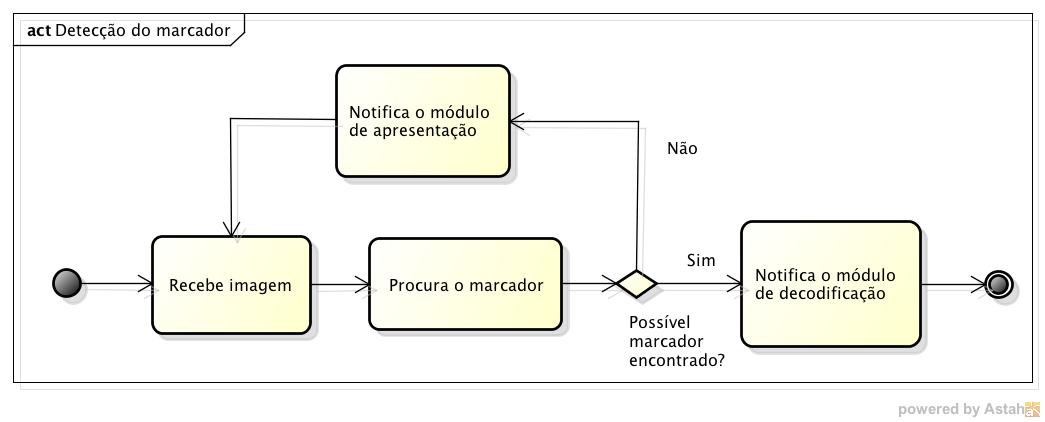
\includegraphics[width=0.9\textwidth]{figuras/processo_deteccao.png}
	%		\end{center}
	%		\caption{Etapas do processo de reconhecimento.}
	%		\label{fig:etapas_decodificacao}
	%	\end{figure}
	%	
	%\end{frame}
	
	% ------------- Módulo de Decodificação  -------------
	
	%\begin{frame}
	%	\frametitle{Módulo de decodificação}
	%	
	%	\begin{itemize}
	%	  \item Módulo responsável pela decodificação do QRCode;
	%	  \item Utilização de QRCodes para armazenamento do nome do dispositivo;
	%	  \item Descarte das imagens recebidas do módulo de reconhecimento enquanto
	%	  		há uma execução em andamento;
	%	  \item Oferece suporte a outras aplicações de decodificação de QRCodes. 
	%	\end{itemize}
	%\end{frame}
	%\begin{frame}
	%	\frametitle{Módulo de decodificação}
	%	
	%	\begin{figure}[htb]
	%		\begin{center}
	%				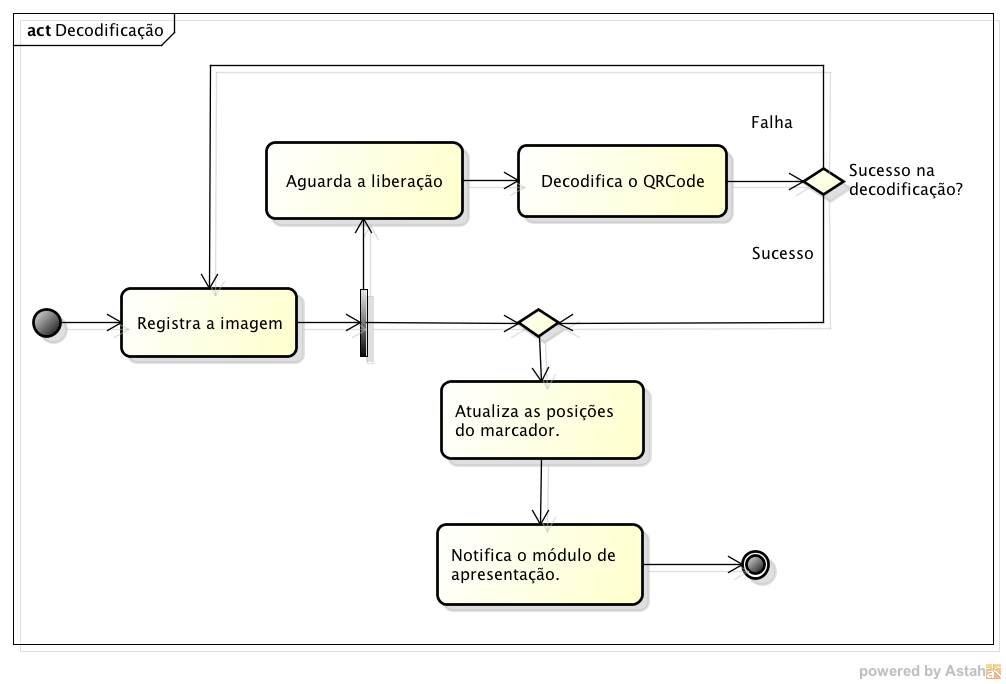
\includegraphics[width=0.8\textwidth]{figuras/processo_decodificacao.png}
	%		\end{center}
	%		\caption{Etapas do processo de decodificação.}
	%		\label{fig:etapas_decodificacao}
	%	\end{figure}
		
	%\end{frame}
	
	% ------------- Módulo de integração -------------
	
	%\begin{frame}
	%	\frametitle{Módulo de integração}
	%	
	%	\begin{itemize}
	%	  \item Este módulo é responsável pela integração da ARHydra com a 
	%			Hydra;
	%	  \item Comunicação através de \emph{drivers};
	%	  \item Criação do \emph{Hydra Driver};
	%	  \item Atualização dos dispositivos à cada minuto. 
	%	\end{itemize}
	%\end{frame}
	
	% ------------- Módulo de apresentação -------------
	%\begin{frame}
	%	\frametitle{Módulo de apresentação}
	%	
	%		Este módulo fica responsável pela apresentação do objeto virtual
	%		ao usuário, contendo todos os recursos disponíveis do dispositivo 
	%		selecionado.
	%	
	%\end{frame}
	
	\begin{frame}
		\frametitle{Visualização do objeto virtual}
		\begin{figure}[htb]
			\begin{center}
					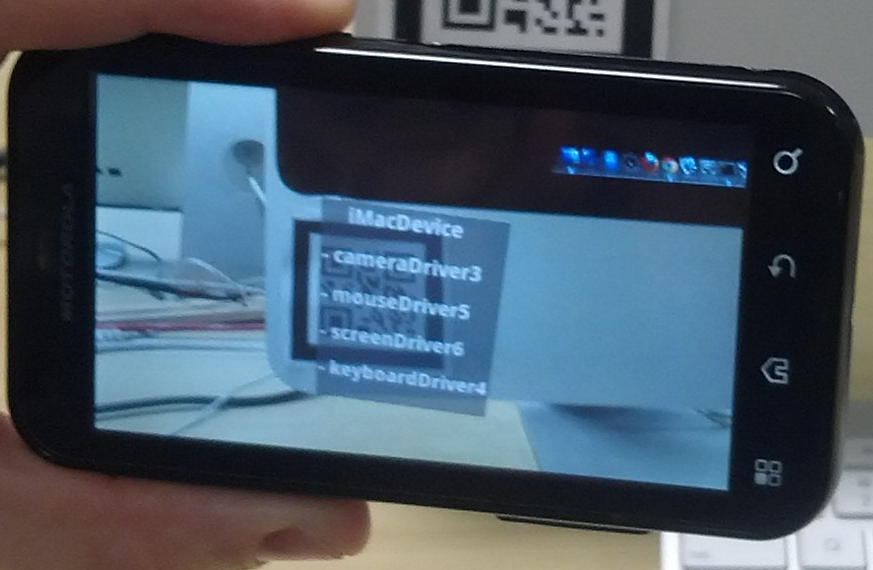
\includegraphics[width=0.75\textwidth]{figuras/objeto_virtual.png}
			\end{center}
		\end{figure}		
	\end{frame}
	
	\begin{frame}
		\frametitle{Apresentação de todos os recursos}
		\begin{figure}[htb]
			\begin{center}
				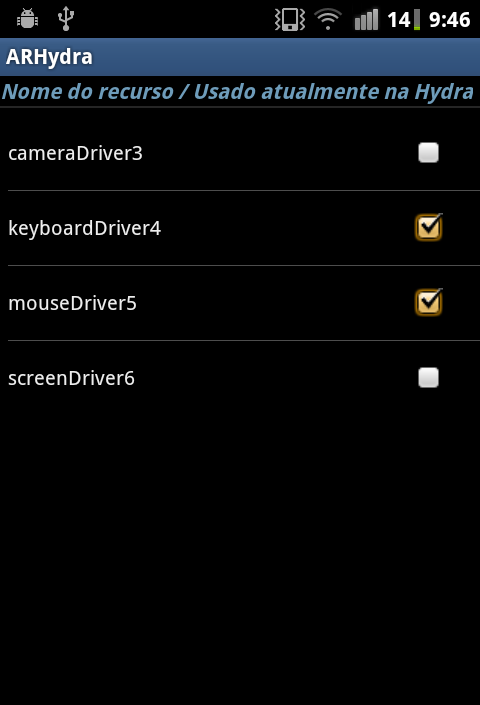
\includegraphics[width=0.45\textwidth]{figuras/listagem_recursos.png}
			\end{center}
		\end{figure}
	\end{frame}
	
	%\begin{frame}
	%	\frametitle{Visualização do objeto virtual}
	%	\begin{figure}[htb]
	%		\begin{center}
	%				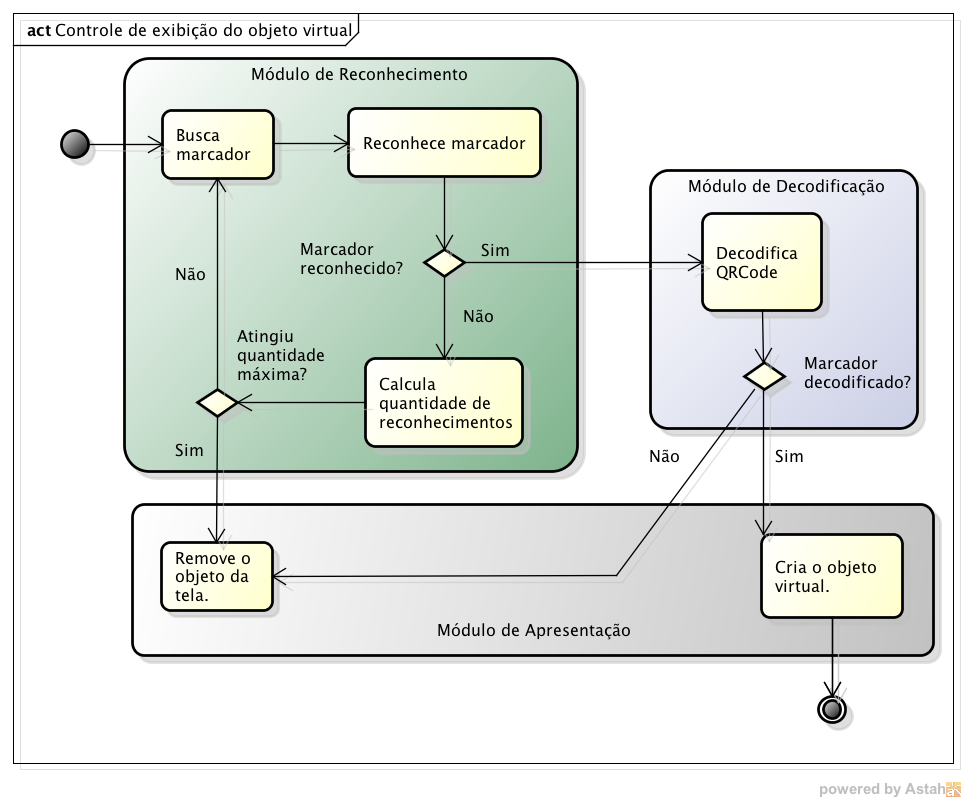
\includegraphics[width=0.8\textwidth]{figuras/condicoes_objeto.png}
	%		\end{center}
	%		\caption{Condições para visualização do objeto virtual.}
	%		\label{fig:condicoes_apresentacao}
	%	\end{figure}
	%\end{frame}
	
	
% ------------- Teste e Resultados -------------

\section{Testes e resultados}

	\begin{frame}
		\frametitle{Testes}
		
		Objetivos:
		\begin{itemize}
			\item	Medir as diferenças no desempenho e qualidade na obtenção das imagens 
					da aplicação ARHydra utilizando dois \emph{smartphones}	diferentes;  
			\item 	Utilização de duas aplicações voltadas para a decodificação do QRCode
					para verificar aquela que apresentava melhores resultados; 	
			\item 	Verificar o nível de tolerância a falhas do QRCode que melhor se aplica
					na aplicação ARHydra.  	
		\end{itemize}
	\end{frame}	

	\begin{frame}
	\frametitle{Marcador utilizado}
		\begin{figure}[htb]
			\begin{center}
					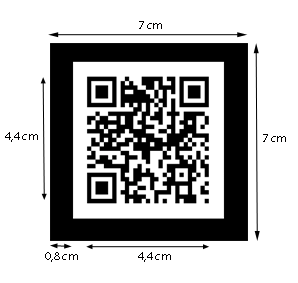
\includegraphics[width=0.6\textwidth]{figuras/dimensoes_marcador.png}
			\end{center}
		\end{figure}
	\end{frame}


	\begin{frame}
		\frametitle{Tempo de reconhecimento}
		
		O tempo de reconhecimento é composto pelo tempo gasto na identificação do marcador,
		decodificação do QRCode, obtenção e apresentação das informações do dispositivo. 
	\end{frame}
	
	\begin{frame}
		\frametitle{Tipos de medições}
		Foram feitas três tipos de medições:
		\begin{itemize}
		  \item Tempo médio do primeiro reconhecimento;
		  \item Tempo médio de recorrência;
		  \item Tempo médio de reconhecimento ao perder o marcador.
		\end{itemize}
	\end{frame}
		  
	\begin{frame}
		\frametitle{Medição de taxas}
		
		\begin{itemize}
		  \item Taxas de erro;
		  \item Taxa de não decodificação.
		\end{itemize}
	\end{frame}
	
	\begin{frame}
		\frametitle{Realização dos testes}
		\begin{itemize}
		  \item Foram analisadas cinco distâncias variada de de 50 centímetros à 1 metro;
		  \item Para cada novo conjunto de testes a distância era aumentada em 10 centímtros;
		  \item Esse valor correspondia a distância entre o marcador e o \emph{smartphone}. 
		\end{itemize}
		
	\end{frame}
	
	%\begin{frame}
	%	\frametitle{Teste de desempenho e qualidade na obtenção da imagem}
	%	
	%	Foram executadas:			
	%	\begin{itemize}
	%	  \item 20 medições para a primeira aparição;
	%	  \item 200 medições para as recorrências;
	%	  \item 50 medições para o reconhecimento ao perder o marcador.
	%	\end{itemize}
	%	
	%\end{frame}
	
	
	%\begin{frame}
	%	\frametitle{Teste de desempenho e qualidade na obtenção da imagem}
	%	\begin{figure}[htb]
	%		\begin{center}
	%				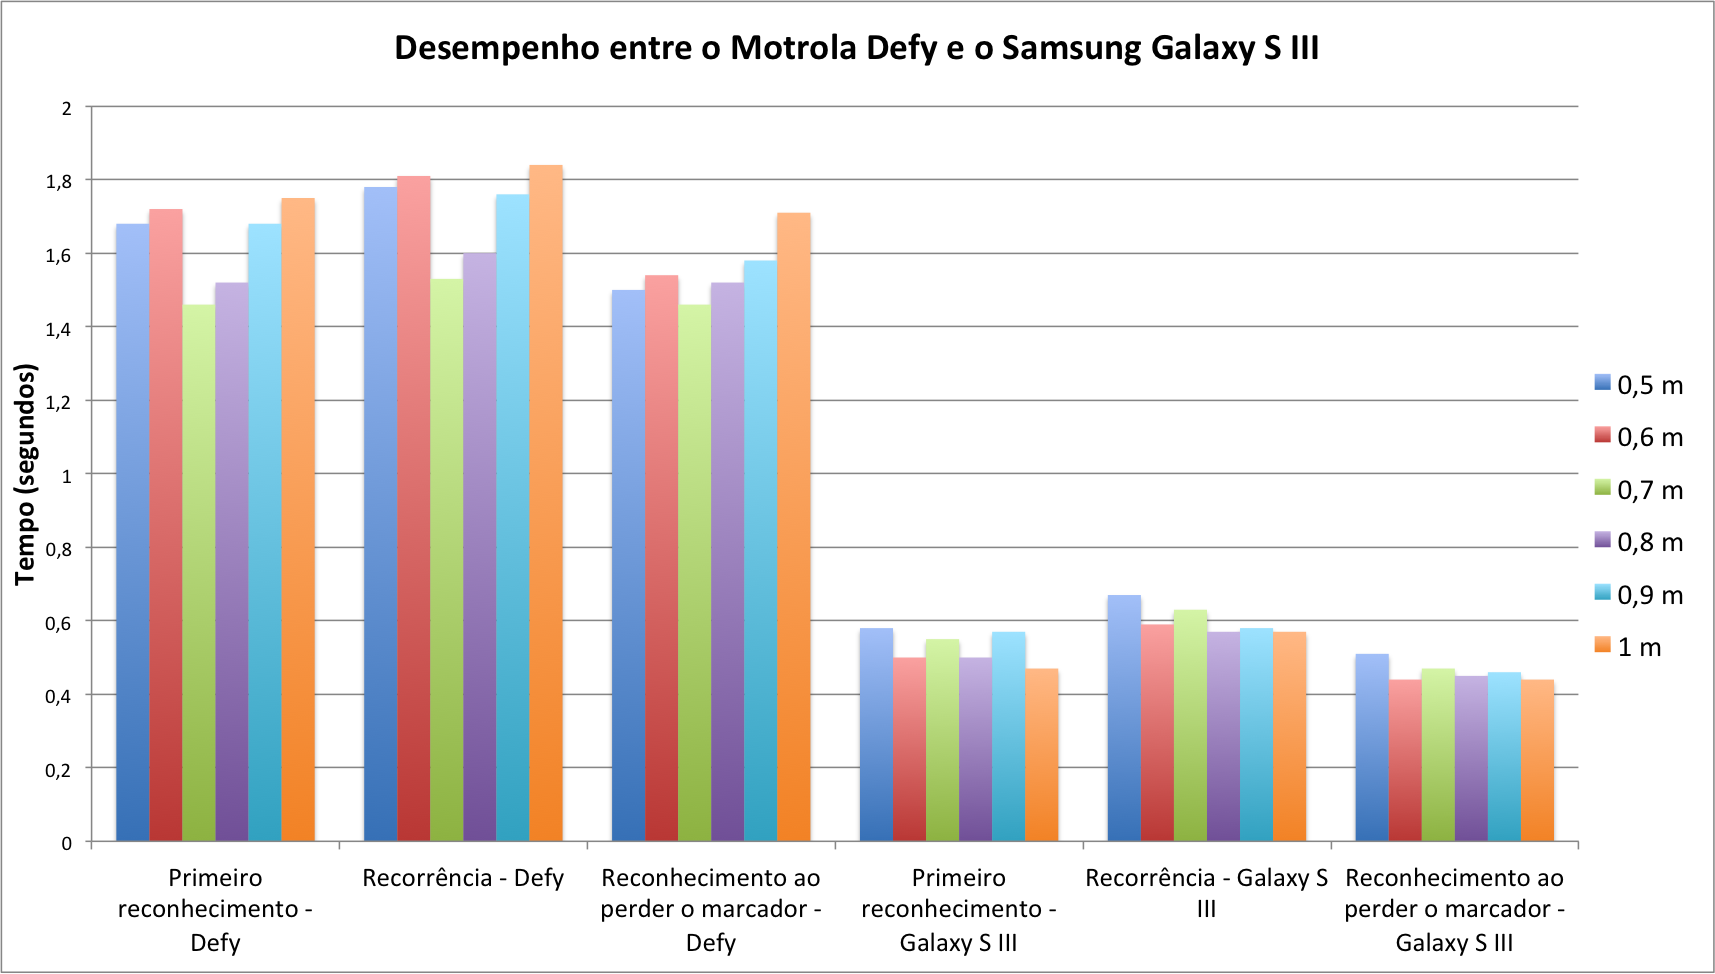
\includegraphics[width=0.9\textwidth]{figuras/grafico_desempenho.png}
	%		\end{center}
	%	\end{figure}
	%\end{frame}
	
	\begin{frame}
		\frametitle{Teste de desempenho}
		
		\begin{itemize}
		  \item Tempos médios do primeiro reconhecimento;
		  \item Foram realizadas 20 medições para o cálculo do tempo médio de primeiro reconhecimento. 
		\end{itemize}
		
				
		\begin{figure}[htb]
			\begin{center}
					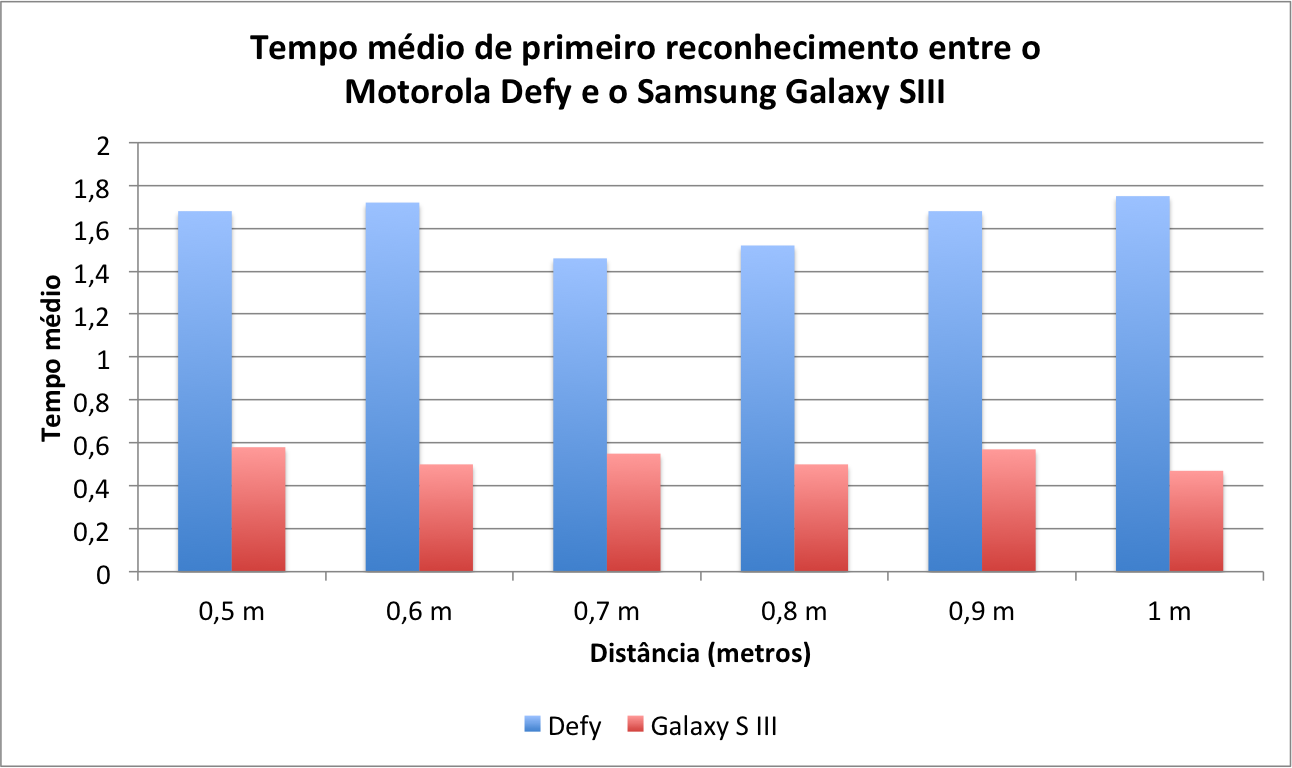
\includegraphics[width=0.85\textwidth]{figuras/grafico_des_primeiro.png}
			\end{center}
		\end{figure}
	\end{frame}
	
	\begin{frame}
		\frametitle{Teste de desempenho}
		
		\begin{itemize}
			\item Tempos médios de recorrência;
			\item Foram realizadas 200 medições para o cálculo do tempo médio de recorrência.
		\end{itemize}
				
		\begin{figure}[htb]
			\begin{center}
					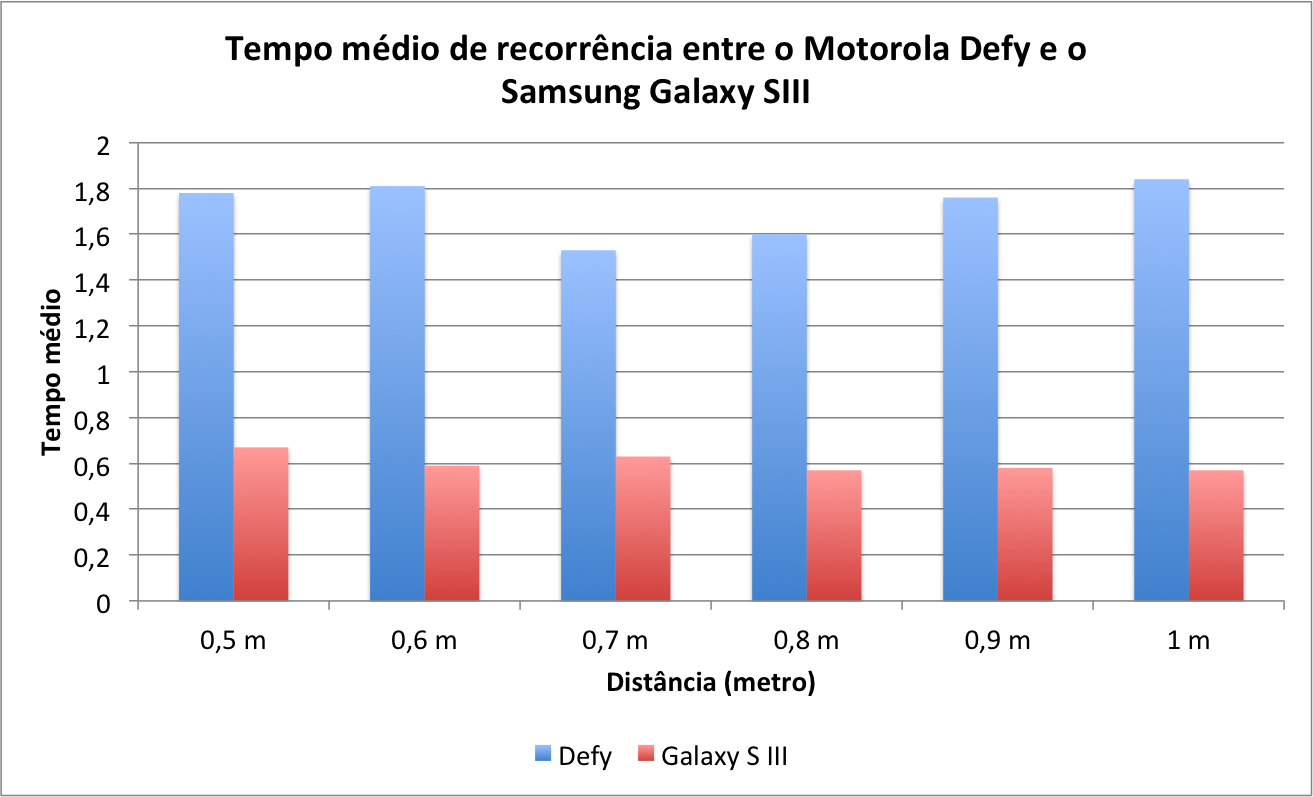
\includegraphics[width=0.85\textwidth]{figuras/grafico_des_recorrencia.png}
			\end{center}
		\end{figure}
	\end{frame}
	
	\begin{frame}
		\frametitle{Teste de desempenho}
		
		\begin{itemize}
		  \item Tempos médios de reconhecimento ao perder o marcador;
		  \item Foram realizadas 50 medições para o cálculo do tempo médio de reconhecimento ao
		  		perder o marcador. 
		\end{itemize}
		
				
		\begin{figure}[htb]
			\begin{center}
					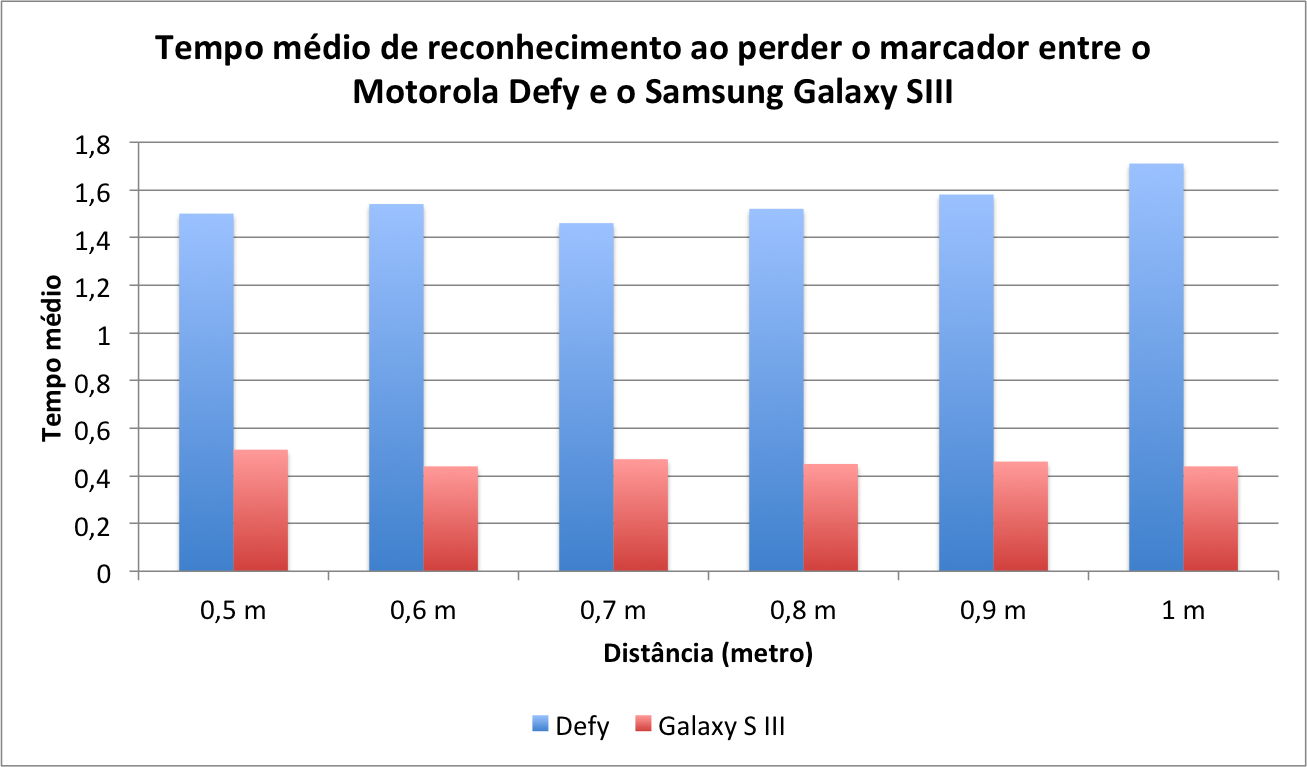
\includegraphics[width=0.85\textwidth]{figuras/grafico_des_perda.png}
			\end{center}
		\end{figure}
	\end{frame}
	
	\begin{frame}
		\frametitle{Qualidade na obtenção da imagem}
		
		Taxa de erros
		
		\begin{figure}[htb]
			\begin{center}
					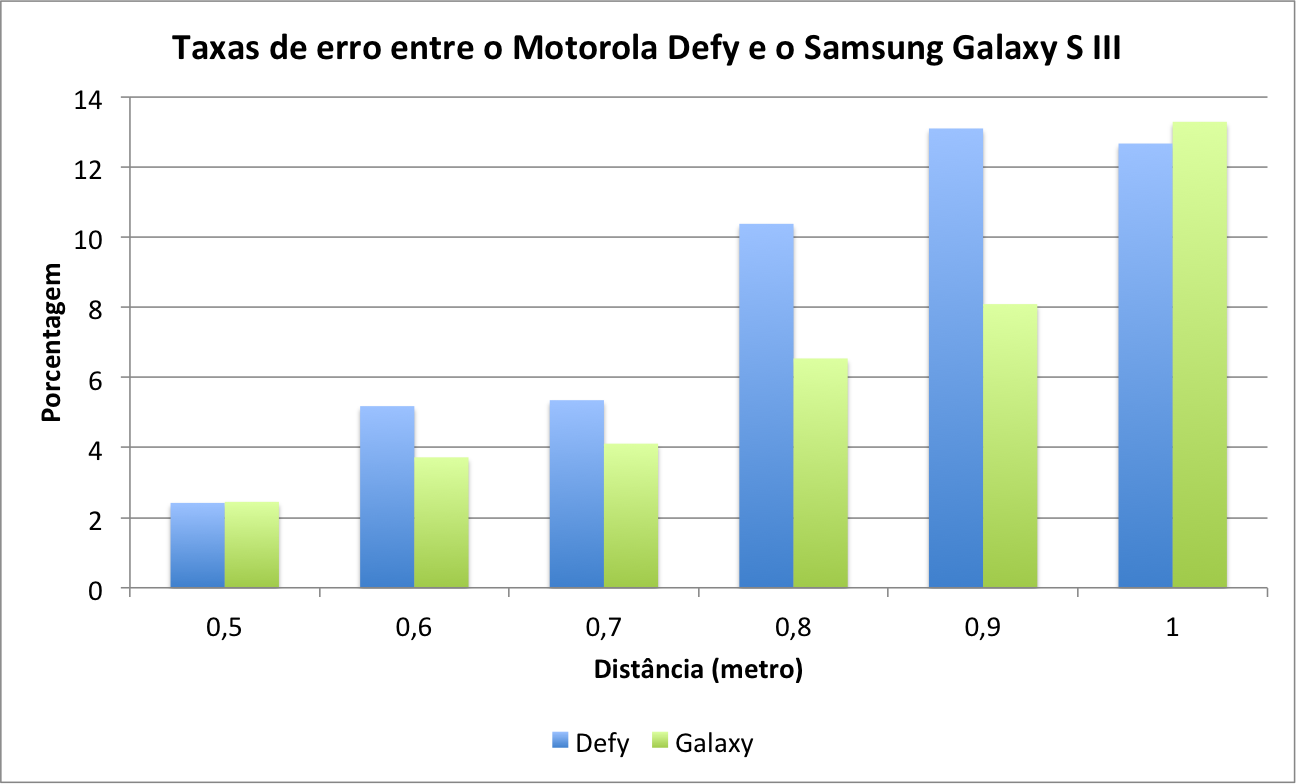
\includegraphics[width=0.85\textwidth]{figuras/taxa_erro_qualidade.png}
			\end{center}
			\caption{Dimensões do marcador.}
			\label{fig:marcador_testes}
		\end{figure}
	\end{frame}
	
	\begin{frame}
		\frametitle{Qualidade na obtenção da imagem}
		
		Taxa de não decodificação
		
		\begin{figure}[htb]
			\begin{center}
					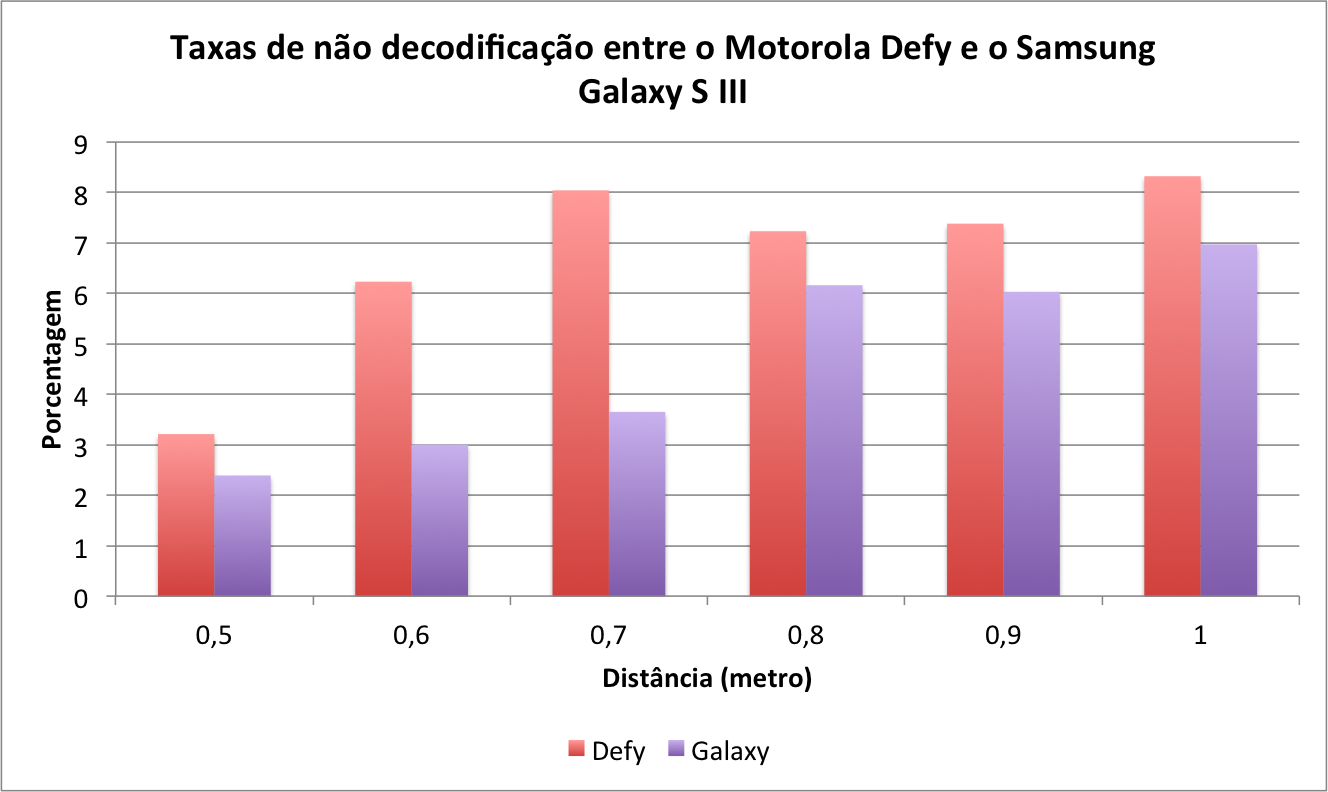
\includegraphics[width=0.85\textwidth]{figuras/taxa_decodificacao_qualidade.png}
			\end{center}
		\end{figure}
	\end{frame}
	
	
	\begin{frame}
		\frametitle{Escolha da melhor aplicação testada para decodificação do QRCode}
		
		\begin{itemize}
		  \item Duas aplicações testadas ZBar e ZXing;
		  \item Foram executados 500 medições para cada distância analisada. 
		\end{itemize}
		
		 \begin{figure}[htb]
			\begin{center}
					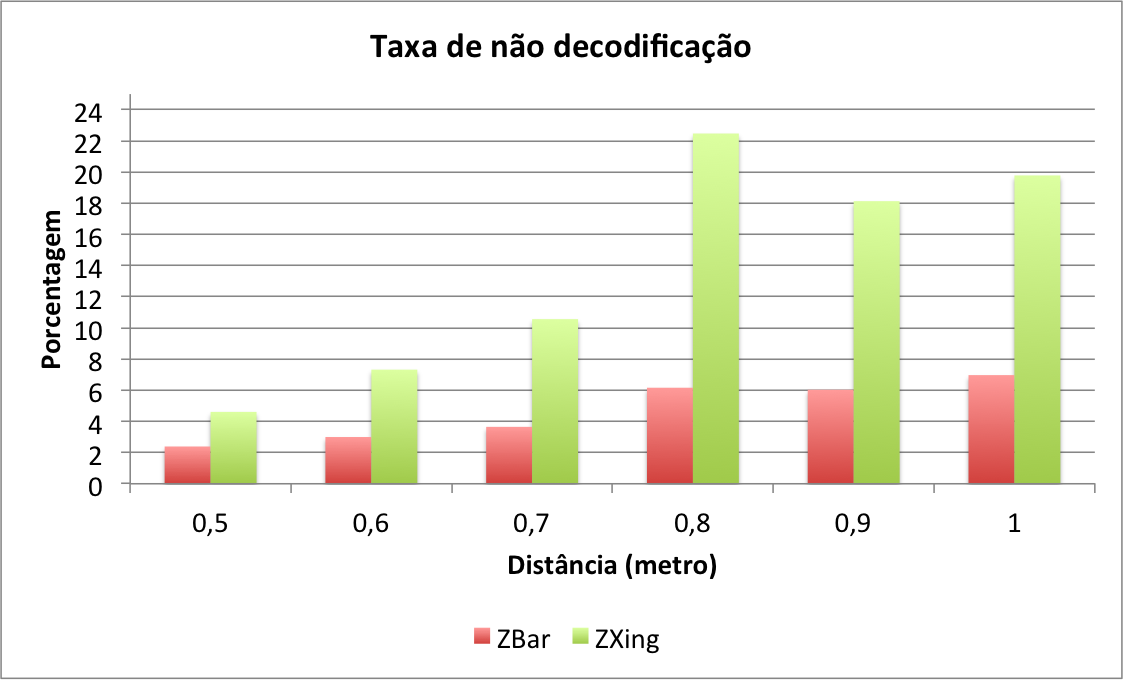
\includegraphics[width=0.85\textwidth]{figuras/grafico_suporte.png}
			\end{center}
		\end{figure}
	\end{frame}
	
	\begin{frame}
		\frametitle{Influência da tolerância a falhas do QRCode}
		
		Foram realizadas 500 medições para cada distância, repetidas para todos os níveis.
		
		\begin{figure}[htb]
			\begin{center}
					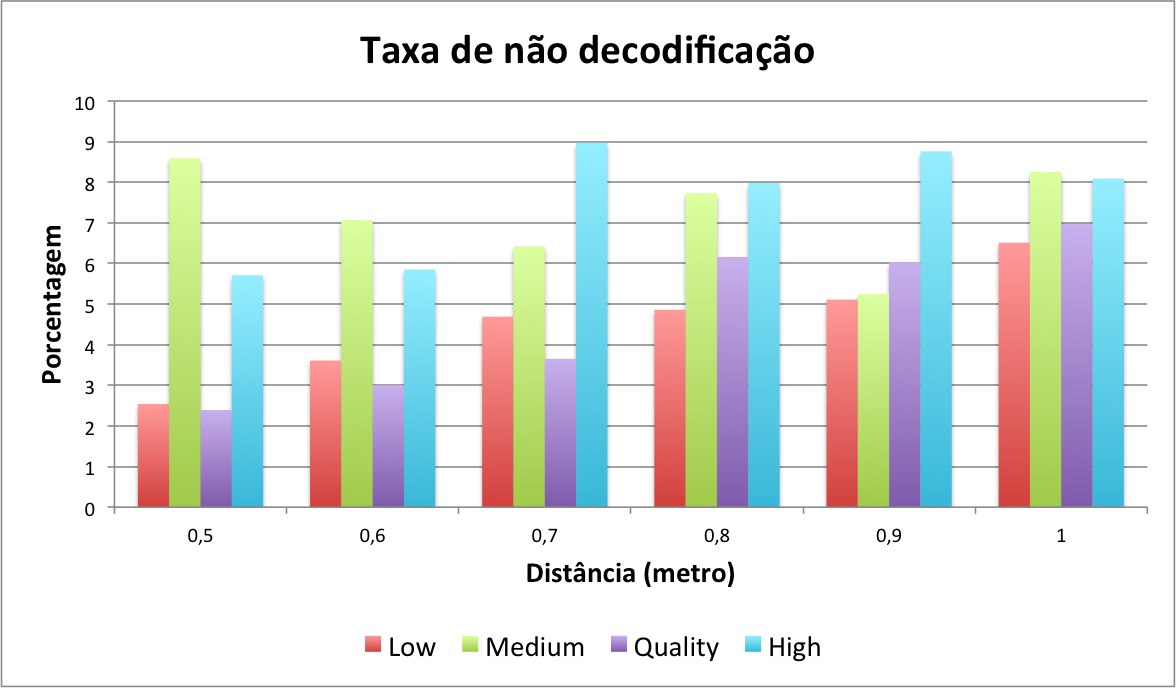
\includegraphics[width=0.85\textwidth]{figuras/grafico_nivel_decode.png}
			\end{center}
		\end{figure}
	\end{frame}

% ------------- Trabalhos futuros -------------
\section{Conclusão}
\begin{frame}
	\frametitle{Conclusão}
	
	\begin{itemize}
	  \item A ARHydra auxilia o usuário na localização, visualização e redirecionamento
	  		dos recursos presentes no ambiente inteligente;
	  \item A aplicação é sensível as condições do ambiente e dispositivo (iluminação do 
	  		ambiente, qualidade na imagem obtida, dentre outros fatores) para uma correta
	  		execução;
	  \item Mostrou ser uma boa forma de interação com a Hydra. 
	\end{itemize}
	
\end{frame}

% ------------- Trabalhos futuros -------------

\section{Trabalhos futuros}
	\begin{frame}
		\frametitle{Trabalhos futuros}
		\begin{itemize}
		  \item Múltiplos marcadores
		  \item Aplicação de filtros
		  \item Cache de reconhecimento
		\end{itemize}
	\end{frame}


% ------------- Referências -------------
\section{Referências}

\frame[allowframebreaks]{
  \frametitle{Referências}
  \bibliographystyle{plain}
  \bibliography{bibliografia}
}
\nocite{mark21Century,ubiSmartSpace,paulDourish,almeida,buzeto_11,ronaldAzuma,milgram,hirzer,forman}


% ------------- Fim -------------
\section{ }
\begin{frame}
    \frametitle{ }
	\centerline{Obrigado.} 
\end{frame}

\begin{frame}
    \frametitle{Perguntas? }
    \begin{figure}[h]
		\centering 
\includegraphics[scale=.55]{figuras/perguntas.jpg}
	\end{figure}
\end{frame}

\end{document}